\documentclass[10pt,paper=letter]{scrartcl}
\usepackage[alttitle]{cjquines}

\begin{document}

\title{VCSMS PRIME}
\subtitle{Program for Inducing Mathematical Excellence}
\author{Session 9: Coordinates}
\date{October 12, 2017}

\maketitle
\setlength{\unitlength}{1in}
\begin{picture}(0,0)
  \put(5.5,0.5){\hbox{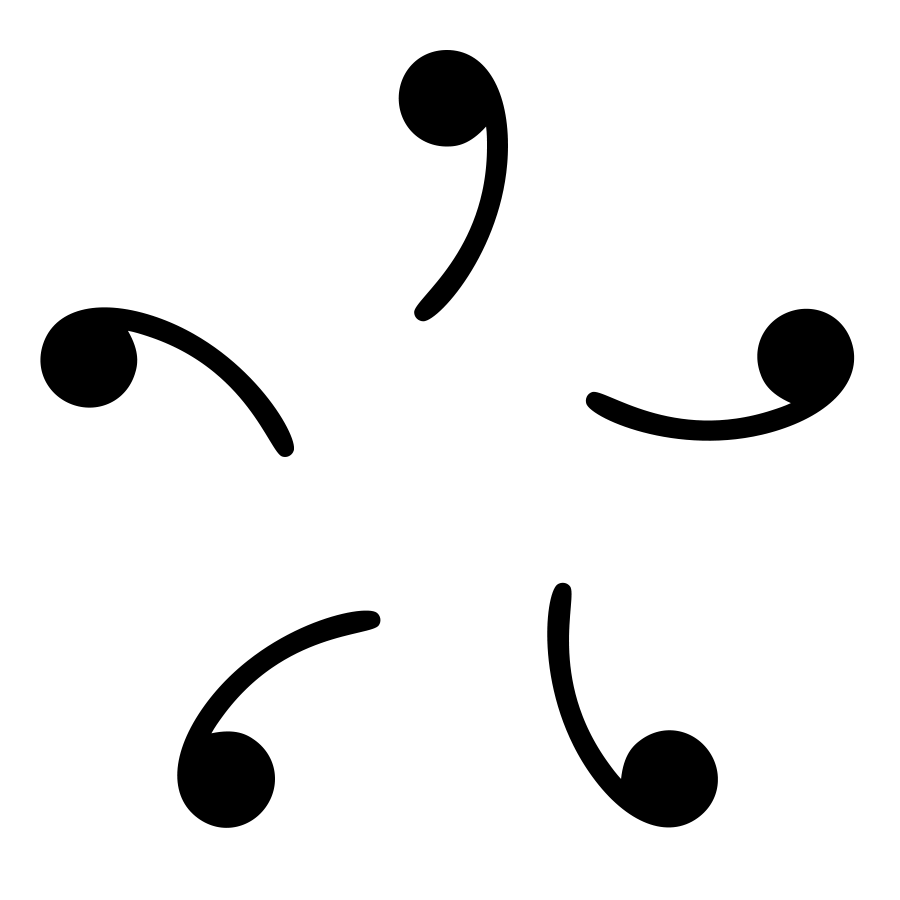
\includegraphics[width=0.9in]{logo.png}}}
\end{picture}
\vspace{-3.5em}

\subsubsection*{Lecture problems}

\begin{enumerate}
  \item In triangle $ABC$, $D$ is the midpoint of $BC$, $E$ is on segment $AC$ such that $AE : EC = 1 : 2$, and $AD$ and $BE$ intersect at $G$. Line $CG$ meets $AB$ at $F$. Find the ratio $CG : GF$.
  \item In triangle $ABC$, $D$ is the midpoint of $BC$, $E$ and $F$ are on $AC$ and $AB$ respectively such that $AE : EC = 1 : 3$ and $AF : FB = 1 : 3$. Let $DE$ and $CF$ intersect at $G$. Compute $CG : GF$.
  \item (AI19) The lengths of the two legs of a right triangle are in the ratio of $7$ : $24$. The distance between its incenter and its circumcenter is $1$. Find its area.
  \item (AI1) The vertices of a triangle are at the points $(0, 0)$, $(a, b)$ and $(2016 - 2a, 0)$, where $a > 0$. If $(a, b)$ is on the line $y = 4x$, find the value(s) of $a$ that maximizes the triangle's area.
  \item (AI10) A line intersects the $y$-axis, the line $y = 2x + 2$, and the $x$-axis at the points $A, B,$ and $C,$ respectively. If segment $AC$ has a length of $4\sqrt{2}$ units and $B$ lies in the first quadrant and is the midpoint of segment $AC$, find the equation of the line in slope-intercept form.
  \item What is the length of the shortest path from $(2, 4)$ to $(6, 2)$ that touches both the $x$- and $y$-axes?
  \item (HMMT 2014) Let $ABC$ be an acute triangle with circumcenter $O$ such that $AB = 4, AC = 5$ and $BC = 6$. Let $D$ be the foot of the altitude from $A$ to $BC$ and let $E$ be the intersection of $AO$ and $BC$. Suppose that $X$ is on $BC$ between $D$ and $E$ such that there is a point $Y$ on $AD$ satisfying $XY || AO$ and $YO \perp AX$. Determine the length of $BX$.
  \item (QIII3) Let $G$ be the set of ordered pairs $(x, y)$ such that $(x, y)$ is the midpoint of $(-3, 2)$ and some point on $\del{x+3}^2 + \del{y-1}^2 = 4$. What is the largest possible distance between any two points in $G$?
  \item A line with slope $1$ is drawn through the focus of the parabola $x^2 - 2y + 1 = 0$, intersecting its directrix at a point $X$. What is the sum of the slopes of the two tangent lines from $X$ to the parabola?
  \item Let $A(2, -1)$, $B(5, -3)$, and $C$ be a point on $y = x^2$. What is the maximum value of $BC - AC$?
\end{enumerate}

\subsubsection*{Mass points}

\begin{itemize}
  \item Ceva's and Menelaus' are simple consequences of mass point geometry. There are two treatments: the classical treatment, and the vectorial treatment. We'll do both, but the important idea is that the masses on both sides balance. 
  \item Problem 1: Mass $2$ to $A$, $1$ to $B$ and $1$ to $C$ works, so $G$ has a mass of $4$. The ratio is $3 : 1$. Alternatively, $D = \frac12B + \frac12C$ and $E = \frac23A + \frac13C$. Point $G$ lies on both $AD$ and $BE$ so $G = \frac12A + \frac12D = \frac14B + \frac34E$. Subtracting $C$ gives $G-\frac14C = \frac34F$ by balancing masses.
  \item Problem 2: We use the vectorial treatment. We have $D = \frac12B + \frac12C$, $E = \frac34A + \frac14C$, $F = \frac34A + \frac14B$. Then $G = kD + (1-k)E = mC + (1-m)F$, and we can solve: $A$ gives $m=k$ and $B$ gives $k = \frac13$, which shows $G = \frac13C + \frac23F$, thus $CG : GF = 2 : 1$.
  \item Problem 3: Let $AB = 7, BC = 24, CA = 25$. We can find the lengths $BD, AD, AI, CI$ using classical mass points and the angle bisector theorem: mass $24$ on $A$, mass $25$ on $B$, mass $7$ on $C$. Then $IO$ is a median in $AIC$, use Stewart's.
\end{itemize}

\newpage

\subsubsection*{Cartesian plane}
% cartesian bashing: area, collinearity, determinants, distance points to points, distance points to lines

\begin{itemize}
  \item Manipulating lines and slopes should be second-nature by now. Shoelace formula, distance between two points, and distance from a point to a line are important. We can treat points as vectors and use ratios.
  \item Problem 4: $(a, b)$ on $y = 4x$ means $b = 4a$. Shoelace formula and maximize a quadratic.
  \item Problem 5: $B$ is the midpoint of the hypotenuse of a right triangle, so $BO$ must have length $2\sqrt2$ units. Set $B(x, 2x+2)$ and use distance formula, then reflect.
  \item Problem 6: Reflection again! Reflect $(2, 4)$ about the $y$-axis and $(6, 2)$ about the $x$-axis, then what are the distances needed?
  \item Problem 7: Let $D$ be the origin. Scale by four to eliminate fractions. Find circumradius to find distance from $O$ to $BC$ to find $O$, which is above the midpoint of $BC$. Find $E$. Set $X = rA$ and $Y = rO$ (ratios are important!) and use the perpendicular condition, which is just slopes.
\end{itemize}

\subsubsection*{Conics}

\begin{itemize}
  \item Conics are a way of thinking: each one is a locus. The parabola is a locus of points equidistant to the focus and the directrix, the ellipse the locus of points with constant sum of distances to foci, the hyperbola the locus of points with constant difference of distances to foci.
  \item The focus of $y = ax^2$ is $\del{0, \dfrac1{4a}}$ and its directrix is $y = -\dfrac1{4a}$. Just translate and rotate. Its range is from its vertex upward.
  \item Problem 8: Set $G$ is a circle with half the radius.
  \item Problem 9: The focus is $(0, 1)$ and the directrix is the $x$-axis, then $X(-1, 0)$. Let $x = my - 1$ be a line through $X$, so its slope is $1/m$. Then substitute in the equation, the quadratic in terms of $y$ should have only one solution, which means it has discriminant zero. This is common trick for tangent to a conic.
  \item Problem 10: Consider the loci of points where $BC - AC$ is constant, a hyperbola; the maximum is when it degenerates to a line through the foci. Then it's just the distance between the foci.
\end{itemize}

\end{document}
